\section{Mockups}

\subsection{ Pantalla Principal de Selección de Rol}
\begin{samepage}\small
Esta pantalla es la puerta de entrada al ecosistema de Argos. Su diseño en modo oscuro (dark mode) establece un tono moderno y profesional desde el primer contacto. La interfaz está diseñada para ser extremadamente simple, guiando a los tres tipos de usuario a su respectivo flujo de trabajo sin ninguna ambigüedad, lo cual es fundamental para una buena primera impresión.
\begin{figure}[H]
	\centering
	\IfFileExists{./Media/Mockups/Page Main.png}{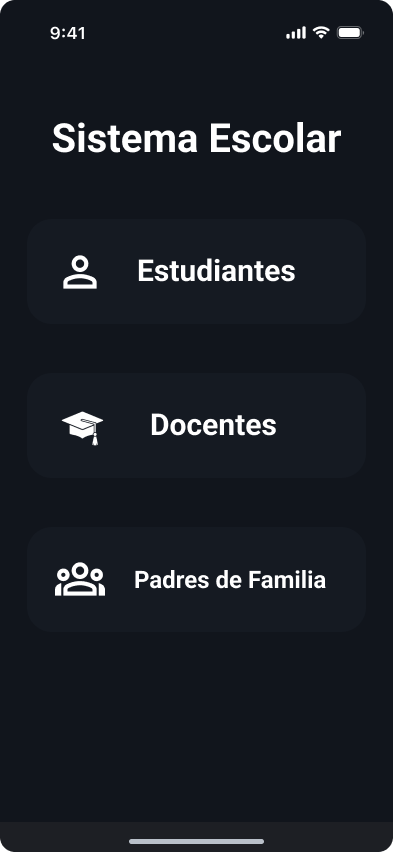
\includegraphics[width=0.28\textwidth]{./Media/Mockups/Page Main.png}}{\fbox{\parbox{0.28\textwidth}{\centering Imagen ``Page Main.png'' no disponible}}}
	\caption{Mockup de la pantalla de selección de rol.}\label{fig:mk-main}
\end{figure}
	\subsubsection*{Análisis de Diseño y Componentes}
	El diseño utiliza una paleta de colores basada en tonos de gris oscuro y carbón, con texto blanco de alto contraste para una legibilidad óptima. Los tres botones de selección para ``Estudiantes'', ``Docentes'' y ``Padres de Familia'' son los únicos elementos interactivos, ocupando un lugar central en la jerarquía visual. Su gran tamaño y esquinas redondeadas los hacen fácilmente pulsables en dispositivos táctiles. La inclusión de iconografía clara y universal (una persona, un birrete, un grupo de personas) junto al texto acelera el reconocimiento del rol.
    
	\subsubsection*{Flujo de Usuario y Funcionalidad}
	El flujo de usuario es intencionadamente lineal: el usuario abre la aplicación, se le presenta esta pantalla, identifica su rol y pulsa el botón correspondiente. Esta acción desencadena una transición a la pantalla de inicio de sesión específica para el perfil seleccionado, creando una experiencia de usuario segmentada y personalizada desde el inicio.
\normalsize\end{samepage}
\clearpage


\subsection{ Pantallas de Inicio de Sesión}
\begin{samepage}\small
Las tres pantallas de inicio de sesión (Estudiante, Docente y Padre de Familia) mantienen una consistencia de diseño casi total para reducir la carga cognitiva del usuario. La única variación significativa es el campo de identificación solicitado, lo cual personaliza el acceso para cada rol. El diseño limpio y enfocado elimina cualquier distracción, centrando al usuario en la tarea de autenticación.
\begin{figure}[H]
	\centering
	\IfFileExists{./Media/Mockups/Login Student.png}{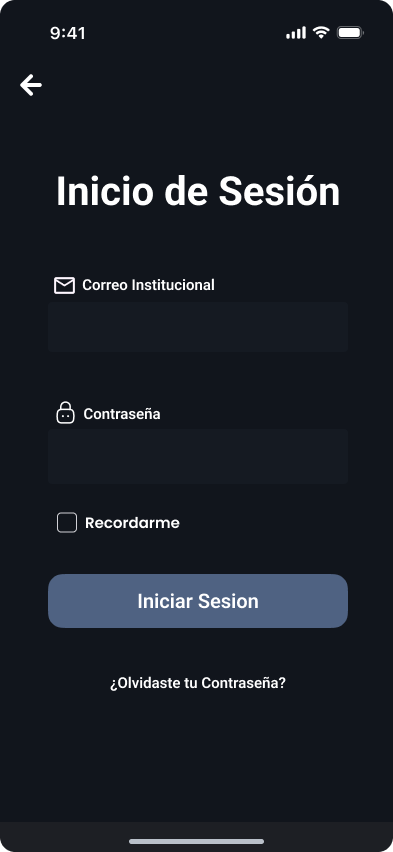
\includegraphics[width=0.22\textwidth]{./Media/Mockups/Login Student.png}}{\fbox{\parbox{0.22\textwidth}{\centering Login Student}}}
	\IfFileExists{./Media/Mockups/Login Teacher.png}{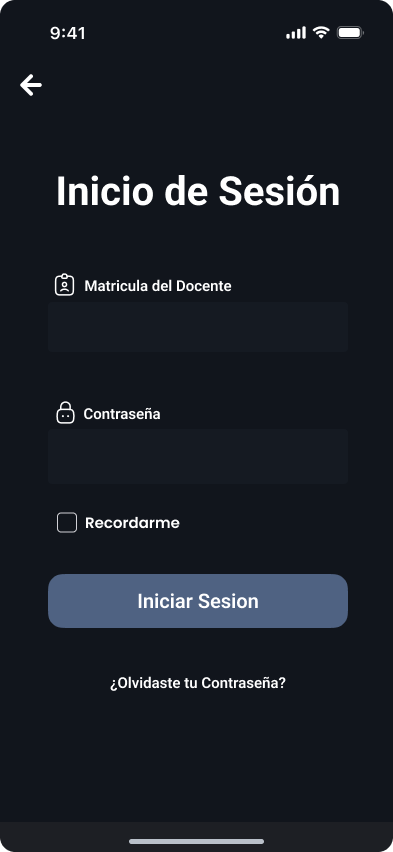
\includegraphics[width=0.22\textwidth]{./Media/Mockups/Login Teacher.png}}{\fbox{\parbox{0.22\textwidth}{\centering Login Teacher}}}
	\IfFileExists{./Media/Mockups/Login Parents.png}{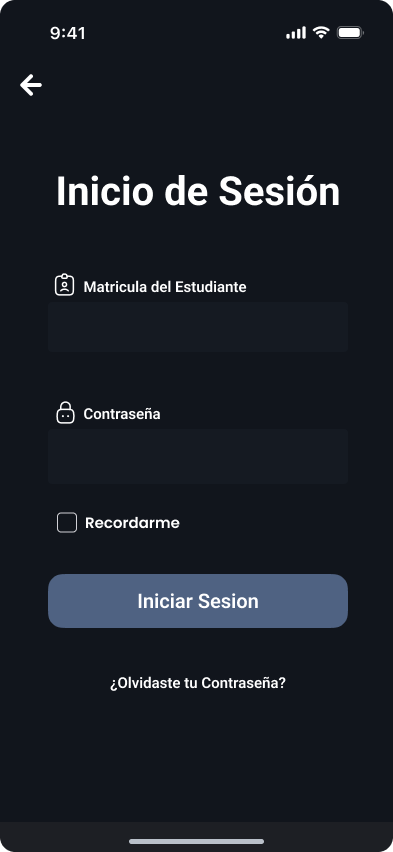
\includegraphics[width=0.22\textwidth]{./Media/Mockups/Login Parents.png}}{\fbox{\parbox{0.22\textwidth}{\centering Login Parents}}}
	\caption{Mockups de las pantallas de inicio de sesión para Estudiante, Docente y Padre de Familia.}\label{fig:mk-logins}
\end{figure}
	\subsubsection*{Análisis de Diseño y Componentes}
	Cada pantalla presenta un título claro, dos campos de entrada con íconos descriptivos, un checkbox para ``Recordarme'', un botón de acción principal (CTA) con un color de acento para destacar, y un enlace secundario para recuperar la contraseña. El campo de identificación cambia según el rol: ``Correo Institucional'' para estudiantes, ``Matrícula del Docente'' para maestros, y ``Matrícula del Estudiante'' para los padres, una decisión de diseño clave para alinear la aplicación con los sistemas de identificación de la institución.
    
	\subsubsection*{Flujo de Usuario y Funcionalidad}
	El usuario introduce sus credenciales y pulsa ``Iniciar Sesión''. El sistema valida la información contra la base de datos. Si la autenticación es exitosa, una pantalla de carga transitoria precede al acceso al panel principal correspondiente a su rol. En caso de error, se mostraría un mensaje específico para guiar al usuario.
\normalsize\end{samepage}
\clearpage

% --- Pantalla de Carga, Home Student, Attendance Student, Profile Student ---
\subsection{ Flujo del Estudiante}
\begin{samepage}\small
El flujo del estudiante está diseñado para ofrecerle una visión completa y clara de su estado académico en relación con la asistencia. La navegación se centra en un menú inferior persistente que le da acceso rápido a las secciones de Inicio, Asistencias y Perfil.
\begin{figure}[H]
	\centering
	\IfFileExists{./Media/Mockups/Home Student.png}{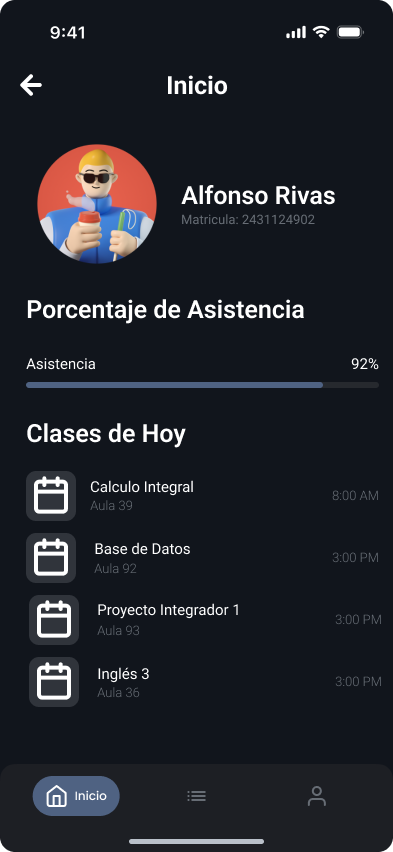
\includegraphics[width=0.22\textwidth]{./Media/Mockups/Home Student.png}}{\fbox{\parbox{0.22\textwidth}{\centering Home Student}}}
	\IfFileExists{./Media/Mockups/Attendance Student.png}{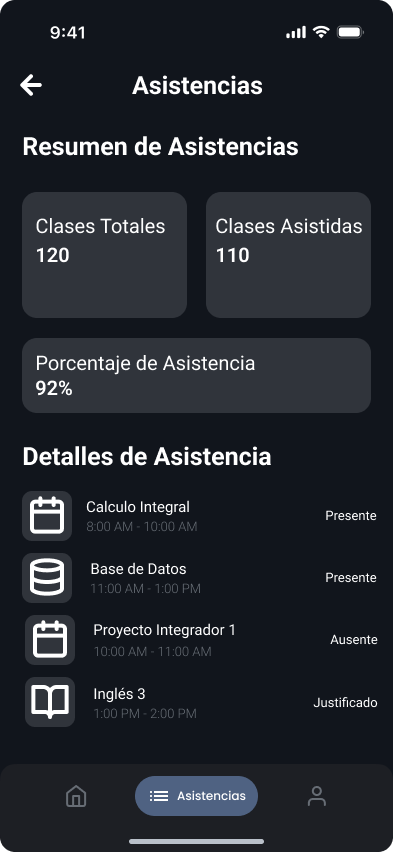
\includegraphics[width=0.22\textwidth]{./Media/Mockups/Attendance Student.png}}{\fbox{\parbox{0.22\textwidth}{\centering Attendance Student}}}
	\IfFileExists{./Media/Mockups/Profile Student.png}{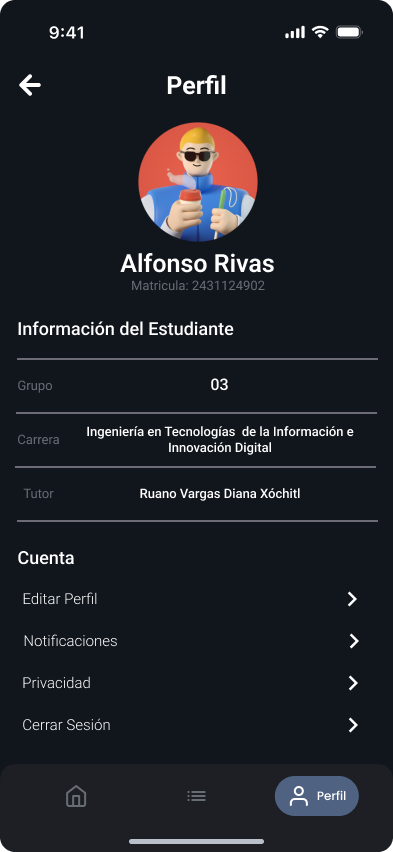
\includegraphics[width=0.22\textwidth]{./Media/Mockups/Profile Student.png}}{\fbox{\parbox{0.22\textwidth}{\centering Profile Student}}}
	\caption{Mockups del flujo del Estudiante: Inicio, Asistencias y Perfil.}\label{fig:mk-student-flow}
\end{figure}
	\subsubsection*{Análisis de Diseño y Componentes}
	La pantalla de \textbf{Inicio} (``Home Student.png'') actúa como un dashboard, personalizando la experiencia con un avatar 3D y mostrando la información más relevante del día: el porcentaje general de asistencia y la lista de clases programadas. La pantalla de \textbf{Asistencias} (``Attendance Student.png'') profundiza en los datos, usando tarjetas de resumen para métricas clave y una lista detallada que clasifica cada clase como ``Presente'', ``Ausente'' o ``Justificado''. La pantalla de \textbf{Perfil} (``Profile Student.png'') agrupa la información personal y las opciones de configuración de la cuenta (Editar Perfil, Notificaciones, etc.) de forma ordenada.
    
	\subsubsection*{Flujo de Usuario y Funcionalidad}
	Desde el inicio, el estudiante puede ver su agenda del día. Si desea más detalles, navega a la sección de Asistencias para un desglose completo. Finalmente, la sección de Perfil le permite gestionar su cuenta y cerrar la sesión de forma segura. El menú de navegación inferior garantiza que estas tres secciones clave estén siempre a un solo toque de distancia.
\normalsize\end{samepage}
\clearpage

% --- Flujo del Docente ---
\subsection{ Flujo del Docente}
\begin{samepage}\small
El flujo del docente está enfocado en la gestión y la eficiencia. Las herramientas están diseñadas para minimizar el tiempo administrativo y facilitar tanto el registro de la asistencia como la consulta de información general de sus grupos.
\begin{figure}[H]
	\centering
	\IfFileExists{./Media/Mockups/Chats.png}{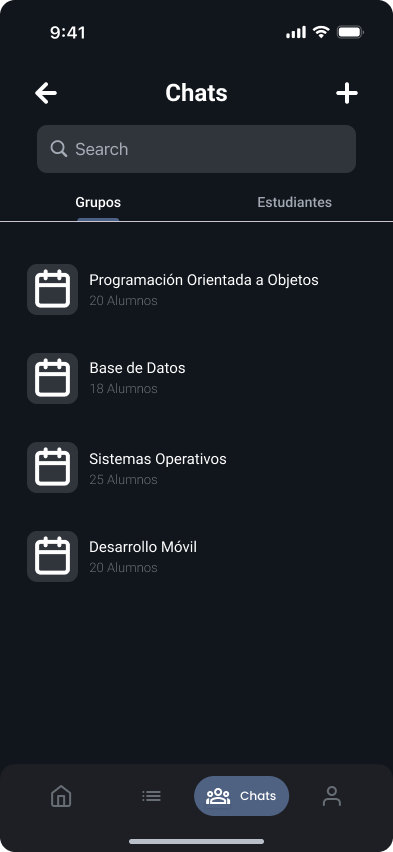
\includegraphics[width=0.22\textwidth]{./Media/Mockups/Chats.png}}{\fbox{\parbox{0.22\textwidth}{\centering Chats}}}
	\IfFileExists{./Media/Mockups/Attendance Pass.png}{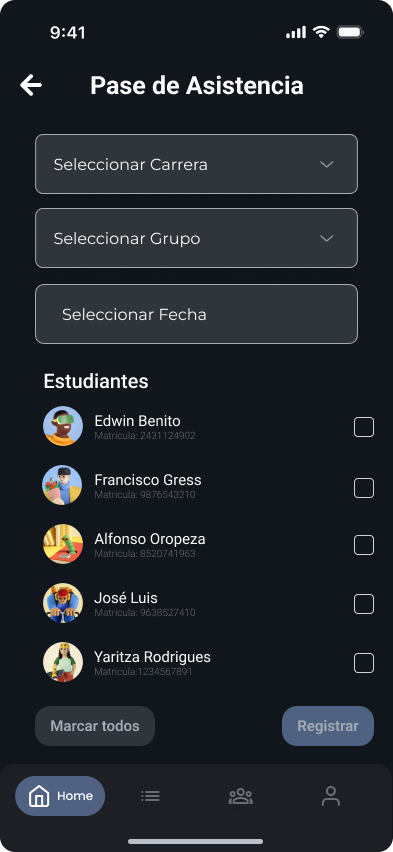
\includegraphics[width=0.22\textwidth]{./Media/Mockups/Attendance Pass.png}}{\fbox{\parbox{0.22\textwidth}{\centering Attendance Pass}}}
	\IfFileExists{./Media/Mockups/Attendance Summary.png}{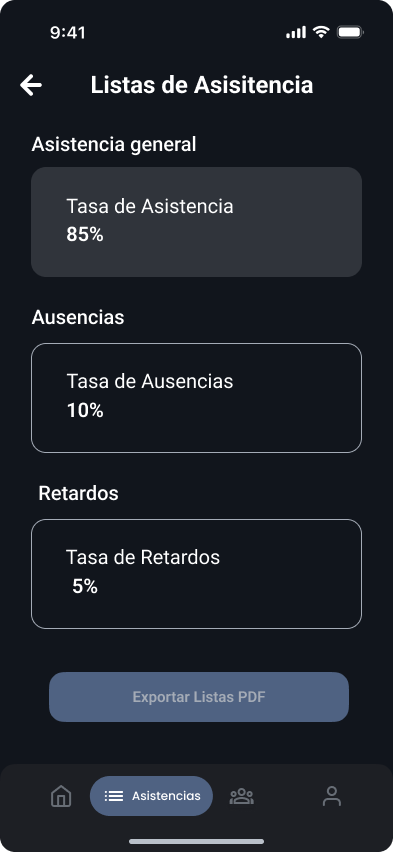
\includegraphics[width=0.22\textwidth]{./Media/Mockups/Attendance Summary.png}}{\fbox{\parbox{0.22\textwidth}{\centering Attendance Summary}}}
	\IfFileExists{./Media/Mockups/Profile Teacher.png}{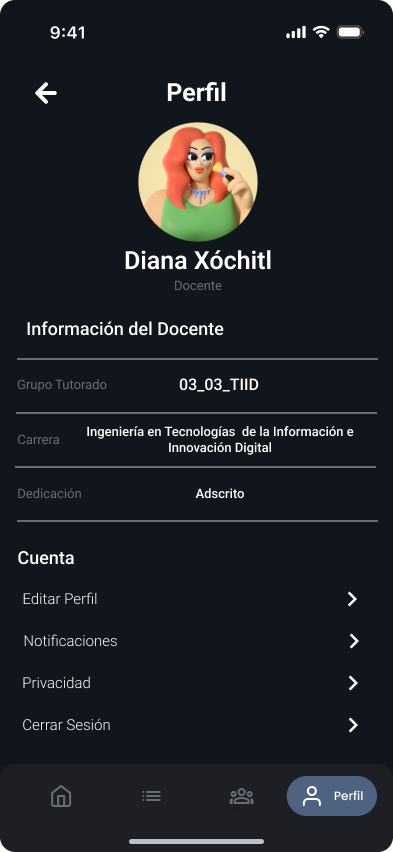
\includegraphics[width=0.22\textwidth]{./Media/Mockups/Profile Teacher.png}}{\fbox{\parbox{0.22\textwidth}{\centering Profile Teacher}}}
	\caption{Mockups del flujo del Docente: Grupos, Pase de Asistencia, Resumen y Perfil.}\label{fig:mk-teacher-flow}
\end{figure}
	\subsubsection*{Análisis de Diseño y Componentes}
	La pantalla de \textbf{Chats/Grupos} (``Chats.png'') funciona como el dashboard principal del docente, listando sus materias y el número de alumnos en cada una. La pantalla de \textbf{Pase de Asistencia} (``Attendance Pass.png'') es puramente funcional, con filtros desplegables y una lista de estudiantes con avatares y checkboxes para un registro rápido. La de \textbf{Resumen de Asistencia} (``Attendance Summary.png'') utiliza tarjetas grandes para mostrar estadísticas globales, como la tasa de asistencia, y un botón claro para exportar los datos. Finalmente, el \textbf{Perfil del Docente} (``Profile Teacher.png'') sigue la misma estructura que el del estudiante para mantener la coherencia.
    
	\subsubsection*{Flujo de Usuario y Funcionalidad}
	El docente inicia en su lista de grupos. Al seleccionar uno, podría ser dirigido al pase de asistencia. Tras registrar, puede navegar a la sección de resúmenes para ver las estadísticas consolidadas y exportar los reportes necesarios. El perfil le permite gestionar su información personal y la configuración de su cuenta.
\normalsize\end{samepage}
\clearpage

% --- Flujo de Padres de Familia ---
\subsection{ Flujo de Padres de Familia}
\begin{samepage}\small
El flujo para los padres de familia está diseñado para ser informativo y directo, proporcionando las herramientas necesarias para un seguimiento efectivo de la asistencia de sus hijos y facilitando la comunicación con la institución.
\begin{figure}[H]
	\centering
	\IfFileExists{./Media/Mockups/Child registration.png}{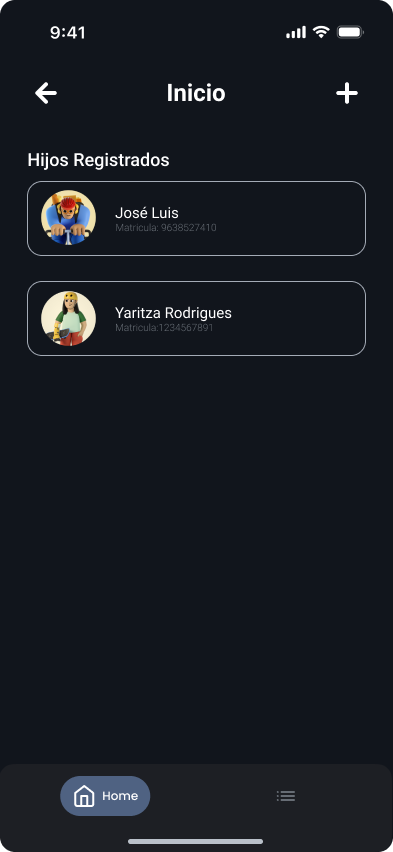
\includegraphics[width=0.22\textwidth]{./Media/Mockups/Child registration.png}}{\fbox{\parbox{0.22\textwidth}{\centering Child registration}}}
	\IfFileExists{./Media/Mockups/Attendance report.png}{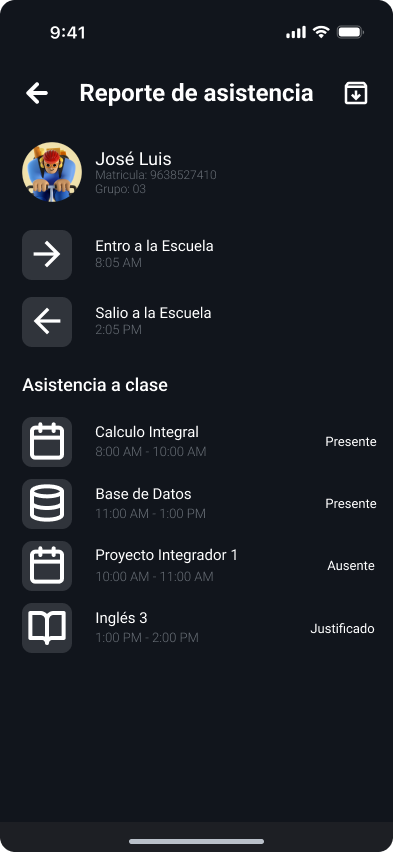
\includegraphics[width=0.22\textwidth]{./Media/Mockups/Attendance report.png}}{\fbox{\parbox{0.22\textwidth}{\centering Attendance report}}}
	\caption{Mockups del flujo de Padres de Familia: Selección de Hijo y Reporte de Asistencia.}\label{fig:mk-parents-flow}
\end{figure}
	\subsubsection*{Análisis de Diseño y Componentes}
	La pantalla de \textbf{Inicio del Padre} (``Child registration.png'') es una lista simple y clara de los ``Hijos Registrados'' bajo su tutela. Cada elemento de la lista muestra el avatar y el nombre completo del estudiante, funcionando como un punto de acceso a la información detallada. La pantalla de \textbf{Reporte de Asistencia} (``Attendance report.png'') presenta un informe diario completo para el hijo seleccionado. Destaca la información de entrada y salida de la escuela, seguida de un desglose detallado de la asistencia a cada clase del día. Un botón de descarga en la esquina superior derecha permite exportar el reporte.
    
	\subsubsection*{Flujo de Usuario y Funcionalidad}
	Al iniciar sesión, el padre ve la lista de sus hijos. Al seleccionar a uno, accede al reporte de asistencia del día actual. Desde allí, puede revisar el cumplimiento del horario escolar y el estatus en cada materia. La función de descarga le permite guardar un registro formal del día.
\normalsize\end{samepage}
\clearpage

% --- Pantalla de Carga Adicional ---
\subsection{ Pantalla de Carga}
\begin{samepage}\small
Finalmente, la pantalla de carga es un componente esencial de la experiencia de usuario que se presenta en transiciones clave. Su diseño final integra el logo de Argos, reforzando la identidad de la marca mientras el sistema procesa información en segundo plano.
\begin{figure}[H]
	\centering
	\IfFileExists{./Media/Mockups/Page Loader.png}{
\includegraphics[width=0.28\textwidth]{./Media/Mockups/Page Loader.png}}{\fbox{\parbox{0.28\textwidth}{\centering Imagen ``Page Loader.png'' no disponible}}}
	\caption{Mockup de la pantalla de carga de la aplicación.}\label{fig:mk-loader}
\end{figure}
	\subsubsection*{Análisis de Diseño y Componentes}
	El diseño es elegante y minimalista. Un círculo central oscuro contiene el isotipo de Argos en blanco, creando un punto focal. Un indicador de actividad sutil (una matriz de puntos) pulsa suavemente debajo, comunicando que la aplicación está activa sin ser visualmente abrumador. El fondo degradado añade una capa de sofisticación al diseño.
    
	\subsubsection*{Flujo de Usuario y Funcionalidad}
	Esta pantalla aparece automáticamente después de que el usuario realiza una acción que requiere tiempo de procesamiento, como iniciar sesión o generar un reporte complejo. Su función es gestionar la percepción del tiempo de espera, asegurando al usuario que su solicitud está siendo procesada y evitando que abandone la aplicación por pensar que se ha bloqueado.
\normalsize\end{samepage}